% Methods chapter
\chapter{Methods}
\label{chap:methods}

This chapter details feature engineering, model architectures, calibration and uncertainty estimation, training and hyperparameter selection, and the evaluation plan, including ablations and error analysis. The dataset is described in Chapter~\ref{chap:dataset}.

\section{Text Preprocessing}
\label{sec:methods-preproc}
We process only participant-authored English messages, already de-identified (Chapter~\ref{chap:dataset}). Preprocessing preserves semantic content while minimizing irreversible transformations:
\begin{itemize}
  \item Normalize whitespace; lowercase except for transformer inputs which retain original casing for cased models.
  \item Replace redaction placeholders (e.g., \verb|<EMAIL:ab12>|) with typed tokens (e.g., \verb|<EMAIL>|) for lexicon features; keep the original placeholders for sequence models to preserve consistency cues.
  \item Tokenization: for TF-IDF and n-grams, use spaCy en\_core\_web\_sm with contractions handled; remove URLs/emails already replaced by placeholders. Lemmatization is enabled. Stopwords are removed for n-grams but retained for LIWC-style counts that rely on function words (first-person pronouns).
  \item Sentence splitting using spaCy; emojis mapped to valence categories where used as features.
\end{itemize}

\section{Feature Engineering}
\label{sec:methods-features}
We compute privacy-safe aggregates at the participant level over a 12-month window prior to PHQ-9 administration. Let \(D_p\) be the set of a participant \(p\)'s messages within the window.

\subsection{Textual Features}
\begin{itemize}
  \item Transformer embeddings: We encode each message using \texttt{roberta-base}. We obtain the \verb|[CLS]|-equivalent pooled representation (mean of last hidden states). User-level embedding is the mean over messages: \(e_p = \frac{1}{|D_p|}\sum_{m \in D_p} f_\theta(m)\). We also compute a temporal mean per month for temporal ablations.
  \item TF-IDF n-grams: character 3--5 grams and word 1--2 grams (min df=5, max features=50k). For the baseline logistic regression, we use these plus lexicon features.
  \item Lexicon counts: LIWC-like categories (affect, negations, first-person singular/plural, social), NRC emotion (anger, fear, joy, sadness, trust, disgust, anticipation, surprise), and VADER sentiment (compound, pos, neg, neu). Counts normalized per 1,000 tokens.
  \item Negations and modifiers: counts of negation tokens and scope-adjusted sentiment flips using a 3-token window.
  \item Pronouns: rates of I/me/my and we/us/our per 1,000 tokens.
\end{itemize}

\subsection{Behavioral and Temporal Features}
Using per-message timestamps in UTC:
\begin{itemize}
  \item Diurnal/circadian: histogram over 24 hours and 7 days; compute entropy and concentration (circular mean resultant length \(R\)). Nighttime activity ratio (00:00--05:59).
  \item Inter-message intervals: log-normal fit parameters (\(\mu, \sigma\)) for \(\log \Delta t\); burstiness \(B = (\sigma - \mu)/(\sigma + \mu)\) on inter-event times; proportion of short gaps (\(<5\) min).
  \item Weekly rhythm stability: autocorrelation at lag 7 days; spectral peak at 1/day and 1/week using Lomb-Scargle.
  \item Proxy login times: first message times per day; distributional stats (median, IQR).
\end{itemize}

\subsection{Interaction Features}
\begin{itemize}
  \item Message length: median, IQR, 90th percentile of token counts; fraction of very short messages (\(\leq 3\) tokens).
  \item Media usage: rates of attachments by type based on flags (images, videos, stickers, voice); binary ever/never plus per-1,000 messages counts.
  \item Response latency: for dyadic threads, estimate participant latency as time from last peer message to participant reply within 24h; summarize by median, IQR, and tail quantiles. Only aggregates retained; no raw conversational sequences are stored.
\end{itemize}

A compact summary of feature groups and definitions is provided in Table~\ref{tab:features-summary}. The feature pipeline DAG is shown in Figure~\ref{fig:feature-dag}.

\begin{figure}[t]
  \centering
  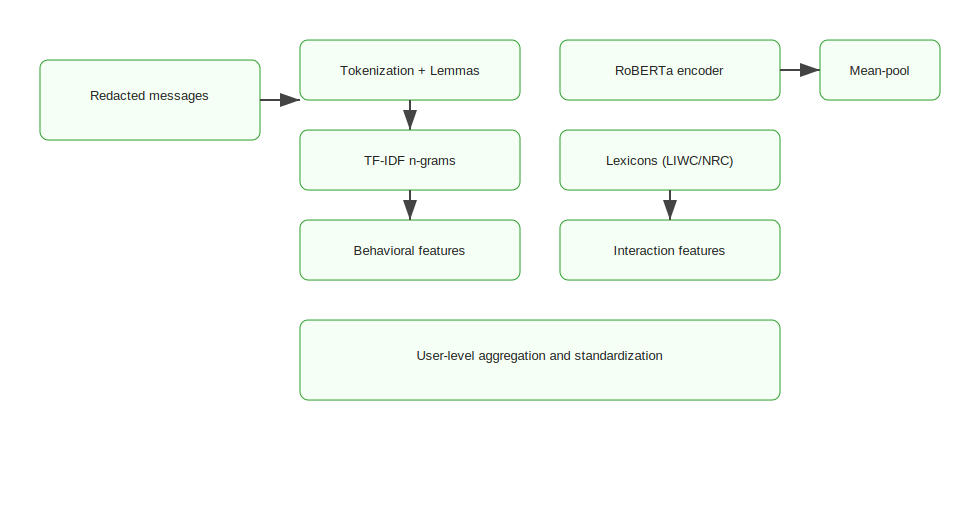
\includegraphics[width=0.95\linewidth]{thesis/figures/feature_dag.svg}
  \caption{Feature extraction pipeline DAG from raw redacted messages to user-level aggregates.}
  \label{fig:feature-dag}
\end{figure}

\section{Models}
\label{sec:methods-models}
\subsection{Baselines}
\begin{itemize}
  \item Logistic regression with L2 penalty on TF-IDF features plus lexicon and interaction aggregates. Solver \verb|liblinear|; class weights balanced.
\end{itemize}

\subsection{Neural Models}
\begin{itemize}
  \item RoBERTa fine-tuning: per-message encoder \texttt{roberta-base} with sequence length 128, learning rate in \([1\times10^{-5}, 5\times10^{-5}]\), batch size 32, 3 epochs. User aggregation by mean pooling of message embeddings; classification head MLP (hidden sizes: [256], dropout 0.2). End-to-end training with random sampling of up to 2,000 messages per user per epoch to cap cost.
  \item Multimodal late fusion: concatenate user-level text embedding with behavioral aggregates and Big Five z-scores; classifier is MLP with layers [128, 64], ReLU, dropout 0.3. We compare early vs late fusion; we adopt late fusion for simplicity and leakage control.
\end{itemize}

\subsection{Calibration and Uncertainty}
\label{sec:methods-calibration}
Post-hoc calibration on validation folds:
\begin{itemize}
  \item Platt scaling (logistic) and isotonic regression applied to validation predictions; select by lower Brier score.
  \item Uncertainty via MC dropout (10 stochastic forward passes at test time) for neural models; also evaluate 3-member deep ensembles where feasible.
\end{itemize}

\section{Training, Hyperparameters, and Reproducibility}
\label{sec:methods-training}
\paragraph{Splits.} We use subject-level stratified splits with no user overlap. Data are split into train/validation/test with proportions 60/20/20 using a fixed random seed (\verb|seed_split = 2025|). We also conduct 5-fold subject-level stratified cross-validation for model selection and confidence intervals (CIs).

\paragraph{Hyperparameter search.} We use Bayesian optimization (TPE) or randomized search with the following ranges: logistic C in \([10^{-4}, 10^{2}]\) log-uniform; TF-IDF max\_features \(\in\{20\text{k}, 50\text{k}\}\); ngram ranges as above; for MLP: hidden sizes \(\in\{[64], [128], [128,64]\}\), dropout \(\in[0.1,0.5]\), L2 \(\in[10^{-6}, 10^{-2}]\); for RoBERTa: learning rate and epochs as above, warmup ratio \(\in[0.0,0.1]\). Early stopping on validation ROC-AUC with patience 3.

\paragraph{Training regime.} Class imbalance addressed with class weights and/or focal loss trials; batch normalization not used. Optimizer: AdamW with weight decay 0.01 for neural models. Gradient clipping at 1.0. Mixed precision training enabled. We fix \verb|numpy|, \verb|torch|, and \verb|sklearn| seeds to 42 for reproducibility and log exact package versions.

\section{Evaluation Plan}
\label{sec:methods-eval}
\paragraph{Metrics.} We report ROC-AUC, PR-AUC, F1 at the Youden-J index threshold (from validation), Brier score, and calibration curves (reliability diagrams). We compute 95\% CIs via non-parametric stratified bootstrap at the user level (1,000 resamples). We report confusion matrices at the selected threshold.

\paragraph{Leakage control.} Splits are at subject level; all feature computations and normalization parameters for TF-IDF and scalers are fit on training folds only and applied to held-out data. Messages within the last 12 months only are used to align with labels.

\paragraph{Ablations.} We run: (a) text-only; (b) behavioral-only; (c) Big Five-only; (d) text + behavioral; (e) full fusion; (f) temporal windows (last 3, 6, 12 months) while keeping label timing fixed.

\subsection{Error analysis}
\label{sec:methods-error-analysis}
We examine calibrated probability distributions and misclassification patterns by subgroups (gender, age bands if collected), feature importances (logistic coefficients, SHAP for MLP), and provide paraphrased, privacy-safe message exemplars synthesized to reflect common failure modes without quoting raw text. Only aggregate statistics are disclosed. See Section~\ref{sec:dataset-ethics} for privacy constraints.

\section{Figures and Tables}
\begin{figure}[t]
  \centering
  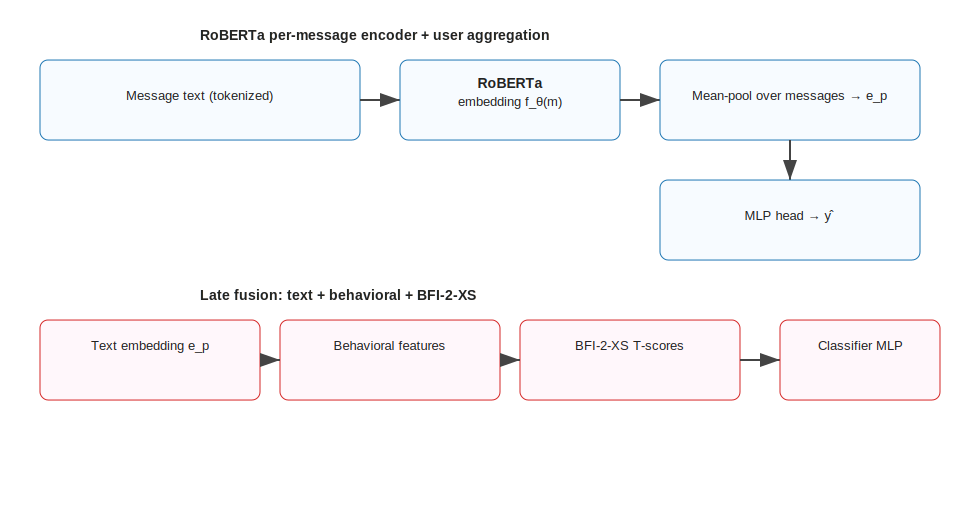
\includegraphics[width=0.9\linewidth]{thesis/figures/model_arch.svg}
  \caption{Model architectures: (left) per-message RoBERTa with user-level aggregation; (right) late-fusion MLP combining text, behavioral, and BFI-2-XS features.}
  \label{fig:model-arch}
\end{figure}

\begin{table}[t]
\centering
\caption{Summary of feature groups and representative definitions. All features are aggregated at the participant level over the 12-month window.}
\label{tab:features-summary}
\begin{tabular}{p{0.20\linewidth}p{0.72\linewidth}}
\toprule
Group & Examples and definitions \\
\midrule
Textual & RoBERTa mean-pooled embeddings; TF-IDF word 1--2g, char 3--5g; LIWC/NRC categories per 1k tokens; VADER sentiment stats; negation counts; first-person pronoun rates \\
Behavioral & Hour-of-day and day-of-week histograms; nighttime ratio; inter-message interval log-normal (mu, sigma); burstiness; weekly autocorrelation; login-time medians \\
Interaction & Message length quantiles; fraction short messages (\(\leq 3\) tokens); media usage flags and rates; response latency med/IQR/tails \\
Personality & BFI-2-XS domain T-scores (O, C, E, A, N) \\
\bottomrule
\end{tabular}
\end{table}



